 
 \begin{center}\begin{large} Practice Problems 5
 \end{large}\end{center}
 \bigskip

\bigskip



\begin{problem}
There are two boxes containing $\{5, 11, 8\}$ and $\{10, 8, 6\}$ white, black, red pencils respectively. One pencil is drawn from each box. What is the probability that the pencils have the same color?
\end{problem}
\bigskip


\begin{problem}
Suppose that you know the answers to 20 questions out of the total 25
questions in the entrance examination, from which you are only asked
3 random questions. What is the probability that you answer all of
the questions?
\end{problem}

\bigskip

\begin{problem}
There are two boxes containing {5, 11} and {10, 8} white, black balls
respectively. First, we take out a ball from each of the boxes. Then, we randomly choose one of them. What is the probability that the
final ball is white?
\end{problem}

\bigskip

\begin{problem}
There are three boxes having 4 white and 6 black balls in each of them.
Suppose we perform the following steps in the given order:
    \begin{enumerate}
        \item[a) ] take out a ball from the first box and put it into the second one,
        \item[b) ] take out a ball from the second box and put it into the third one,
        \item[c) ] take out a ball from the third box and put it into the first one.
    \end{enumerate}
    What is the probability of taking a white ball from the third box (after doing \textit{a)-c)})?
\end{problem}

\bigskip

\begin{problem}
Two factories produce similar weapons and deliver it to the army warehouse. The first factory’s productivity is two times more than that of
the second one. Moreover, $40\%$ of the weapons produced by the first
factory have some defects, while the same indicator is only $16\%$ for
the second factory. We randomly take a weapon from the warehouse,
test it and it appears to have no defects. What is the probability that
the weapon was produced by the first factory?

\end{problem}


\bigskip

\begin{problem}
According to some statistics, $5\%$ of all males and $0.25\%$ of all females
are color-blind. Assuming that the populations of males and females
are equal, what is the probability that a randomly chosen color-blind person is a male?
\end{problem}

\bigskip

\begin{problem}
    Nune uses her car $30\%$ of the time, walks $30\%$ of the time and rides the bus $40\%$ of the time as she goes to work. She is late $10\%$ of the time when she walks, $3\%$ of the time when she drives, and $7\%$ of the time she takes the bus.

\begin{enumerate}
    \item[a) ] What is the probability she took the bus if she was late?
    
    \item[b) ] What is the probability she walked if she is on time?
\end{enumerate}

\end{problem}

\bigskip
\begin{problem}
    On the way to the ACA, your
bus passes through a traffic light. The light cycle of the traffic light is $20$
seconds red, $5$ seconds yellow, and $50$ seconds green. What is the
probability that you will pass under a green light?
\end{problem}

\bigskip

\begin{problem}
After a trip to Garni-Geghard, you bring your camera film to a photography shop. Unfortunately, the shop ruins $4$ photos in a row from your roll which contains $24$ photos. What is the probability that the ruined photos included the
\begin{enumerate}
    \item[a) ] eighth, ninth or tenth photos,
    \item[b) ] eighth, ninth and tenth photos
\end{enumerate}
on the roll (the photos of the Garni Temple)?
\end{problem}

\bigskip

\begin{problem}
    Anush and Nairi are shopping at the mall. They agree to split up for a time and then meet for lunch. They plan to meet in
front of Kinopark between 12:00 and 13:00. The one who arrives first agrees to wait $15$ minutes for the other to arrive. After $15$
minutes, that person will leave and continue shopping. What is the probability that they will meet if each one of them arrives at any time between 12:00 and 13:00?

\textit{Hint: Try to represent the problem on coordinate system, by letting
$x$ denote the time Anush arrives, and $y$, the time Nairi arrives.}
\end{problem}

\bigskip

\begin{problem}
    A line segment is $8$ cm long. Two points are put on the segment at
random locations. What is the probability that the three segments formed by
the two points can make a triangle?
\end{problem}


\bigskip

\begin{problem}
 Vahe added a dot on the   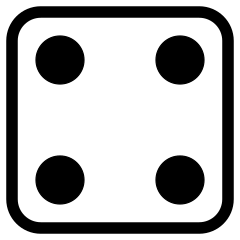
\includegraphics[height=0.9em]{figs/4.png} side of the die, making it 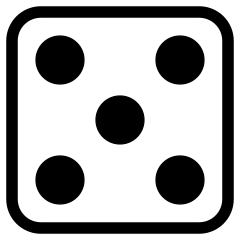
\includegraphics[height=0.9em]{figs/5.png}, and then added two dots on the 
\includegraphics[height=0.9em]{figs/1.png} side, making it 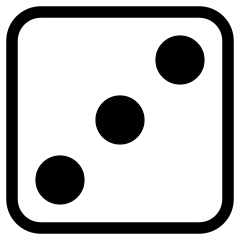
\includegraphics[height=0.9em]{figs/3.png}.
   What is the probability that the outcome of the die is greater than $4$? Find the expectation and variance of the die.
   
\end{problem}


\bigskip

\begin{problem}
   Let $X$ be a random variable with the PDF:
   \[
   f(x) = \begin{cases}
       2x, & 0 \le x \le 1 \\
       0, & \text{otherwise}
   \end{cases}
   \]

   Find the expectation and variance of
   \begin{enumerate}
       \item[a) ] $X$,
       \item[b) ] $2X$,
       \item[c) ] $2X + 7$. 
       
   \end{enumerate}
\end{problem}









% \newpage


% \begin{center}
%     \begin{large}
%         Solutions
%     \end{large}
% \end{center}

% \bigskip


% \begin{solution}
% Let's denote the event of drawing a white, black, red ball from the first box by $W_1$, $B_1$, $R_1$, respectively; and $W_2$, $B_2$, $R_2$ for the second box. Then the event of having two balls of the same color is equivalent to either having two whites, or two blacks, two reds. Therefore,
% \begin{align*}
%     \PP\big((W_1\cap W_2) &\text{ or } (B_1\cap B_2) \text{ or } (R_1\cap R_2) \big) \\&= \PP\big(W_1\cap W_2)+\PP(B_1\cap B_2) +\PP(R_1\cap R_2) \\&= \PP\big(W_1)\PP(W_2)+\PP(B_1)\PP(B_2) +\PP(R_1) \PP(R_2) \\&= \dfrac{5}{24}\cdot \dfrac{10}{24} +  \dfrac{11}{24}\cdot \dfrac{8}{24} +  \dfrac{8}{24}\cdot \dfrac{6}{24} = \dfrac{186}{576} = \dfrac{31}{96} 
% \end{align*}

% An alternative approach would be counting all $24\times 24$ pairs and calculating the probability of one-colored pairs.
% \end{solution}
% \smallskip




% \begin{solution}
% For us to answer all 3 questions correctly, they have to be from the 20 questions we have learned. Let $Q_1, Q_2, Q_3$ be the events of the first, second, third questions being from the questions we know. Then
% \[\PP(Q_1 \cap Q_2 \cap Q_3) = \PP(Q_1)\cdot \PP(Q_2\mid Q_1)\cdot \PP(Q_3 \mid Q_1, Q_2) = \dfrac{20}{25}\dfrac{19}{24}\dfrac{18}{23} = \dfrac{57}{115}. \]

% Or we can just calculate the number of all possible triplets: $C_{25}^{3}$, the number of triplets from questions we know: $C_{20}^{3}$, and divide the latter one by the former:
% \[
% \dfrac{C_{20}^{3}}{C_{25}^{3}} = \dfrac{57}{115}.
% \]
% \end{solution}
% \smallskip


% % \begin{solution}
% % Let's denote the number of unique (distinct) colors of the 3 balls drawn by $X$. ($X$ is a random variable.)

% % Then
% % \[\PP(X\ge 2) = 1 - \PP(X<2) = 1-\PP(X=1),\]
% % so its easier to calculate $\PP(X=1)$ (i.e. the probability that all 3 are of the same color), and subtract it from $1$. The same way as we calculated above, we can see that:
% % \begin{align*}
% %     \PP(X=1) &= \PP\big((W_1\cap W_2 \cap W_3) \text{ or } (B_1\cap B_2 \cap B_3) \text{ or } (R_1\cap R_2 \cap R_3) \big) \\&= \PP\big(W_1\cap W_2\cap W_3)+\PP(B_1\cap B_2\cap B_3) +\PP(R_1\cap R_2\cap R_3) \\&= 0+\dfrac{3}{10}\cdot \dfrac{2}{9} \cdot \dfrac{1}{8} +\dfrac{5}{10}\cdot \dfrac{4}{9} \cdot \dfrac{3}{8}  = \dfrac{66}{720} = \dfrac{11}{120} 
% % \end{align*}
% % \[
% % \PP(X\ge 2) = 1-\dfrac{11}{120}  = \dfrac{109}{120}
% % \]
% % \end{solution}
% % \smallskip



% \begin{solution}
% Let $X$ be 1 if the ball from the first box is white, otherwise 0; and define $Y$ for the second box analogously. Denote by $W$ the event (not an RV!) of choosing a white ball on the final step.

% \begin{align*}
%     \PP(W) &= \PP(W\mid X=1, Y=1)\cdot \PP(X=1,Y=1) \\&+
% \PP(W\mid X=0, Y=1)\cdot \PP(X=0,Y=1)\\&+
% \PP(W\mid X=1, Y=0)\cdot \PP(X=1,Y=0)\\&+
% \PP(W\mid X=0, Y=0)\cdot \PP(X=0,Y=0)
% \end{align*}

% The last case is impossible because we can't choose a white ball from two black balls. Therefore:
% \begin{align*}
%      \PP(W) &= \PP(W\mid X=1, Y=1)\cdot \PP(X=1,Y=1) \\&+
% \PP(W\mid X=0, Y=1)\cdot \PP(X=0,Y=1)\\&+
% \PP(W\mid X=1, Y=0)\cdot \PP(X=1,Y=0)\\&=
% 1\cdot \PP(X=1)\PP(Y=1) +\dfrac{1}{2}\cdot \PP(X=0)\PP(Y=1)+
% \dfrac{1}{2}\cdot \PP(X=1)\PP(Y=0)\\&=
% \dfrac{5}{15}\dfrac{11}{19}+\dfrac{1}{2}\dfrac{10}{15}\dfrac{11}{19}+
% \dfrac{1}{2}\dfrac{5}{15}\dfrac{8}{19}=\dfrac{26}{57}
% \end{align*}
% \end{solution}
% \smallskip




% \begin{solution}
% Let $W_1$ denote the event that we have taken out a white ball from the first box and put into the second one; similarly define $B_1, \dots, W_3$. Also denote by $\tilde{W}$ the event that after steps 1-3, we take a white ball from the third ball.

% We have:
% \begin{align*}
%     &\PP(W_1) = \dfrac{4}{10}= \dfrac{2}{5},\\
%     &\PP(B_1) = \dfrac{6}{10}= \dfrac{3}{5},\\
%     &\PP(W_2) = \PP(W_2\mid W_1)\PP(W_1)+\PP(W_2\mid B_1)\PP(B_1)=\dfrac{5}{11}\dfrac{4}{10}+\dfrac{4}{11}\dfrac{6}{10}=\dfrac{2}{5},\\
%     &\PP(B_2) =1-\PP(W_2)=\dfrac{3}{5}.\\
%     % &\PP(W_3) = \PP(W_3\mid W_2)\PP(W_2)+\PP(W_3\mid B_2)\PP(B_2)=\dfrac{2}{5},\\
%     % &\PP(B_3) =1-\PP(W_3)=\dfrac{3}{5}.\\
% \end{align*}

% The probability of taking out a white ball from the third box depends on the color of the balls put into it (step 2) and taken out from it (step 3). Thus, 
% \begin{align*}
%      \PP(\tilde{W}) &= \PP(\tilde{W}\mid W_2, W_3)\cdot \PP( W_2, W_3) \\&+
%      \PP(\tilde{W}\mid W_2, B_3)\cdot \PP( W_2, B_3) \\&+
%      \PP(\tilde{W}\mid B_2, W_3)\cdot \PP( B_2, W_3) \\&+
%      \PP(\tilde{W}\mid B_2, B_3)\cdot \PP( B_2, B_3) \\&=
%      \PP(\tilde{W}\mid W_2, W_3)\cdot \PP(W_3\mid W_2) \cdot \PP( W_2) \\&+
%      \PP(\tilde{W}\mid W_2, B_3)\cdot \PP(B_3\mid W_2) \cdot \PP( W_2)\\&+
%      \PP(\tilde{W}\mid B_2, W_3)\cdot \PP(W_3\mid B_2) \cdot \PP( B_2) \\&+
%      \PP(\tilde{W}\mid B_2, B_3)\cdot \PP(B_3\mid B_2) \cdot \PP( B_2) \\&=     
% \dfrac{4}{10}\dfrac{5}{11}\dfrac{2}{5} +
% \dfrac{5}{10}\dfrac{6}{11}\dfrac{2}{5} +
% \dfrac{3}{10}\dfrac{4}{11}\dfrac{3}{5} +
% \dfrac{4}{10}\dfrac{7}{11}\dfrac{3}{5} =\dfrac{220}{550} = \dfrac{2}{5}.
% \end{align*}
% \end{solution}
% \smallskip


% \begin{solution}
% Let $F_1$ denote the event that a randomly taken weapon is produced in the first factory, $F_2$ in the second; and let $D$ be the event of it having a defect.

% We have:
% \begin{align*}
%     &\PP(F_1) = \dfrac{2}{3},&\qquad &\PP(F_2) = \dfrac{1}{3}&\\
%     &\PP(D\mid F_1) = 0.4= \dfrac{2}{5},&\qquad &\PP(D\mid F_2) = 0.16= \dfrac{4}{25},
% \end{align*}
% hence 
% \[\PP(D) = \PP(D\mid F_1)\PP(F_1)+\PP(D\mid F_2)\PP(F_2)=\dfrac{8}{25}.\]

% Using Bayes' rule, we get:
% \begin{align*}
%      \PP(F_1 \mid D^C) = \dfrac{\PP(F_1)}{\PP(D^C)}
%      \PP(D^C \mid F_1)=\dfrac{2/3}{17/25}\cdot \dfrac{3}{5}=\dfrac{10}{17}.
% \end{align*}
% \end{solution}
% \smallskip


% \begin{solution}
% Let $F$ denote the event that a randomly taken person is female, $M$ male; and let $C$ be the event they are color-blind.

% We have:
% \begin{align*}
%     &\PP(F)=\PP(M) = 0.5,\\
%     &\PP(C\mid F) = 0.0025,\\
%     &\PP(C\mid M) = 0.05,
% \end{align*}
% hence 
% \[\PP(C) = \PP(C\mid F)\PP(F)+\PP(C\mid M)\PP(M)=0.02625.\]

% Using Bayes' rule, we get:
% \begin{align*}
%      \PP(M \mid C) = \dfrac{\PP(M)}{\PP(C)}
%      \PP(C \mid M)=\dfrac{0.5}{0.02625}\cdot0.05\approx 0.95.
% \end{align*}
% \end{solution}
% \smallskip

% \begin{solution}
%     Let $C, W$ and $B$ denote the events of Nune going by car, walking or bus respectively; and let $L$ denote the event of her being late. Then,
%     \[
%     \displaystyle{\PP(B\mid L) = \frac{\PP(L\mid B) \PP(B)}{\PP(L)}= \frac{0.4 \cdot 0.07}{0.4 \cdot 0.07 +0.3 \cdot 0.03+0.3\cdot 0.1} \approx 0.418.}
%     \]
% \end{solution}
% \smallskip


% \begin{solution}
%     Given that a dart always lands somewhere within the circular area with uniform probability, $|\Omega| = \pi \cdot 5^2 = 25\pi$. Then,

%     \begin{enumerate}
%         \item[a) ] $\PP(\text{circle 1}) = \dfrac{\pi \cdot 1^2}{|\Omega|} = \dfrac{1}{25}$,
        
%         \item[b) ] The total area of two red rings is $(\pi \cdot 4^2 - \pi \cdot 3^2) + (\pi \cdot 2^2 - \pi \cdot 1^2) = 10\pi$, hence  
%         $\PP(\text{red circle}) = \dfrac{10\pi}{|\Omega|} = \dfrac{10}{25} = \dfrac{2}{5}$,
        
%         \item[c) ] $\PP(\text{yellow circle}) = 1 - \PP(\text{red circle}) = \dfrac{3}{5}$.
%     \end{enumerate}
% \end{solution}
% \smallskip

% \newpage
% \begin{solution}

% Let's draw time as an infinite line and mark the $20$, $5$ and $50$ second segments between which the traffic light is constantly switching:
% \\~\\
% {    \centering
%     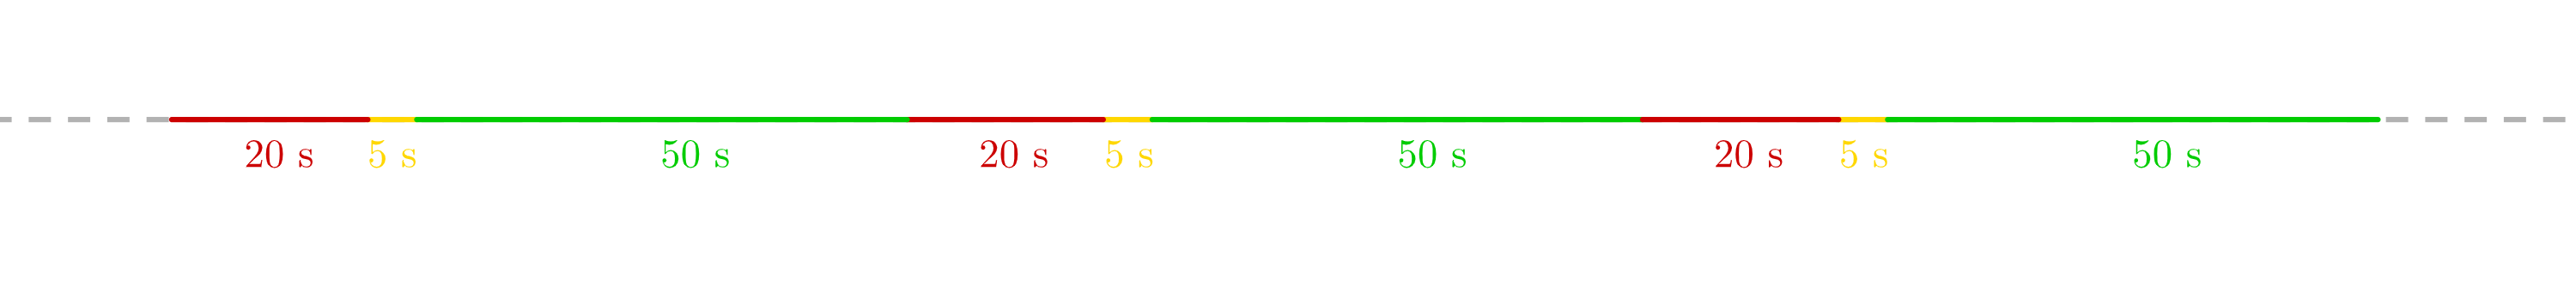
\includegraphics[width=1\linewidth]{figs/solution_light.png}}
% \\~\\
% Because there are $50$ seconds of green in every segment of time with $75$ seconds length, the probability of passing under green light would be $\dfrac{50}{75} = \dfrac{2}{3}$.

% \end{solution}

% \smallskip

% \begin{solution}

% Let $X$ denote the number of the first burned photo in the roll. Clearly, $X$ can have the values $1$ to $21$ each with an equal probability $\dfrac{1}{21}$.

% \begin{enumerate}
%     \item[a) ] For the eighth photo to be burn, $X$ should be one of $\{5, 6, 7, 8\}$; similarly for the ninth it should be one of $\{6, 7, 8, 9\}$; and for the tenth, one of $\{7, 8, 9, 10\}$. We get:
%     \[
%         \PP(X\in \{5, 6, 7, 8\} \cup \{6,7,8,9\}\cup\{7,8, 9, 10\}) = \PP(X\in \{5, 6, 7, 8, 9, 10\}) = \dfrac{6}{21} = \dfrac{2}{7}.
%     \]
    
%     \item[b) ] Similarly, for all three of them to be burned, we have:
%     \[
%         \PP(X\in \{5, 6, 7, 8\} \cap \{6,7,8,9\}\cap\{7,8, 9, 10\}) = \PP(X\in \{7, 8\}) = \dfrac{2}{21}.
%     \]
% \end{enumerate}

% \end{solution}


% \smallskip

% \begin{solution}
% We can represent the problem on a coordinate
% system, by letting $x$ denote the time Anush arrives, and $y$, the time Nairi arrives. Since either of them may arrive at any time within the entire hour, the sample space may be
% represented as the square $\Omega = [0,60]\times [0,60]$. The area of the sample space is, thus, $|\Omega|=60^2=3600$.

% The feasible region is found by representing the 15-minute waiting
% period. There are two cases:
% \begin{enumerate}
%     \item[a) ] If Nairi arrives first, then Anush ($x$) and Nairi ($y$) will meet if $y - x < 15$;
    
%     \item[b) ] If Anush arrives first, then Anush ($x$) and Nairi ($y$) will meet if $x - y < 15$.
% \end{enumerate}

% 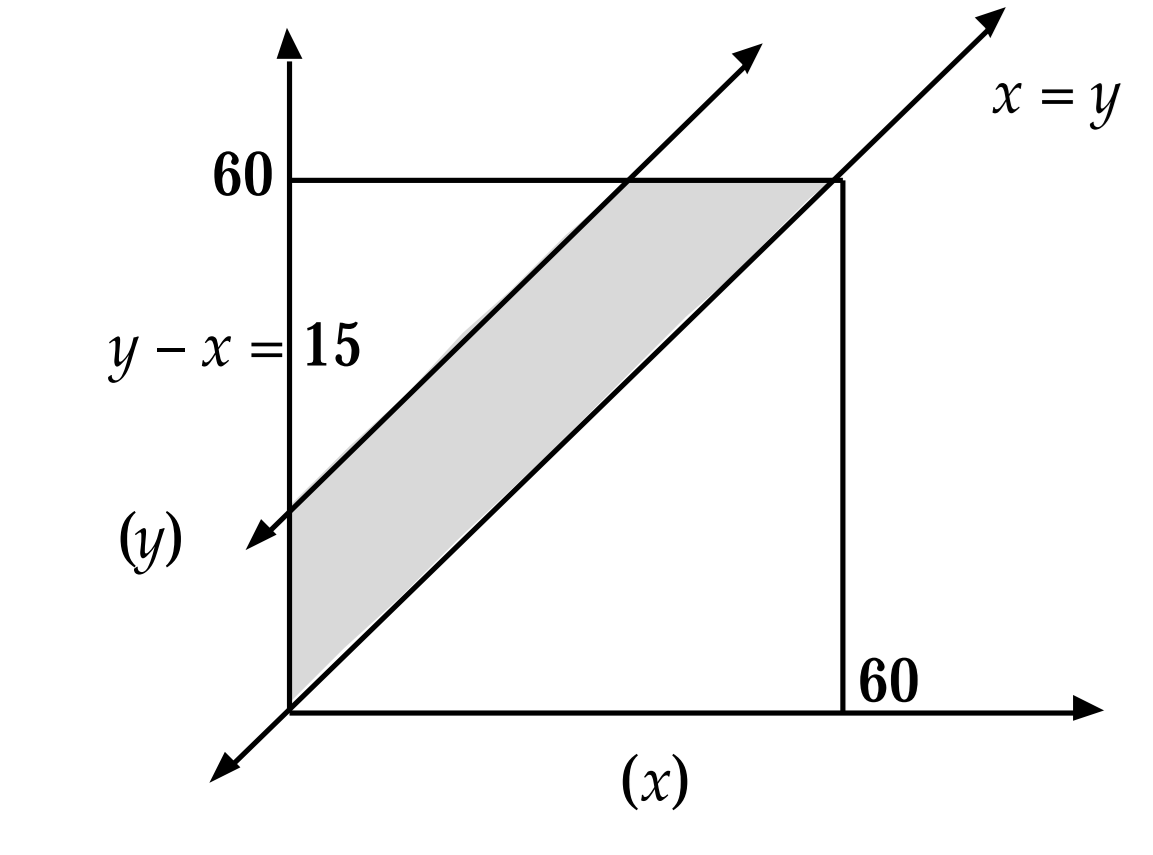
\includegraphics[width=0.4\linewidth]{figs/region2.png}
% 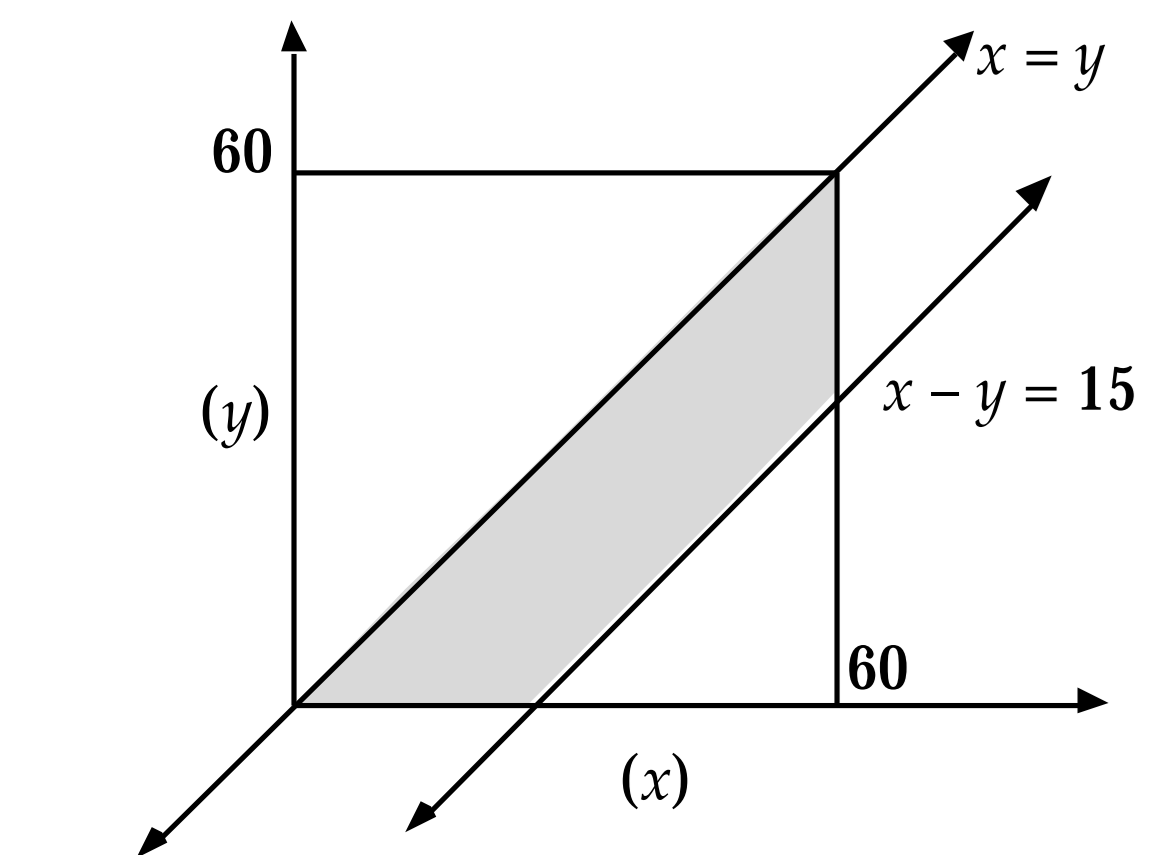
\includegraphics[width=0.4\linewidth]{figs/region1.png}
% \\
% \begin{center}
%     \textit{
% \qquad  a) Nairi arrives first \qquad  \qquad \qquad \quad b) Anush arrives first \qquad\qquad\qquad}
% \end{center}

% \newpage

% The union of the two shaded areas is the feasible region. If the
% arrival times of the two can be represented by a point within
% either shaded area, then they will meet. Calculating the shaded area and dividing it by the area of the sample space, we get:
% \[
% \PP(\text{Nairi and Anush will meet}) = \PP(|x-y|<15) = \dfrac{60^2-45^2}{60^2} = \dfrac{1575}{3600} = 0.4375.
% \]

% \begin{figure}
%     \centering
% 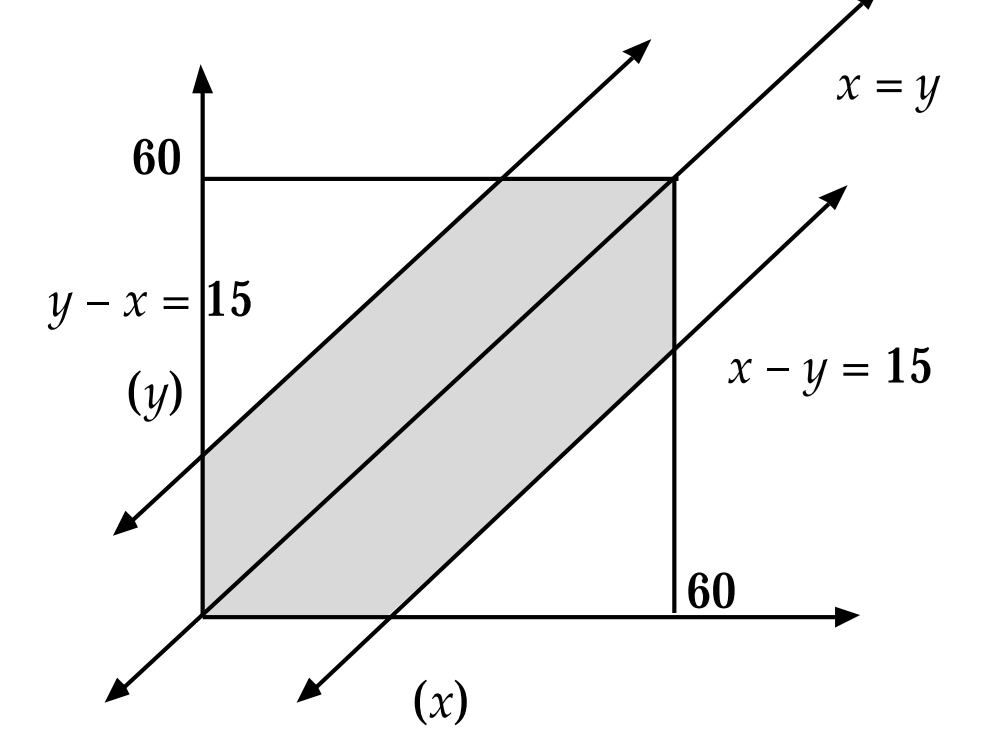
\includegraphics[width=0.4\linewidth]{figs/region3.png}
% \end{figure}

% \end{solution}


% \smallskip

% \begin{solution}

% When we put two points (let's say $B$ and $C$) on a segment (say, $AD=8$) we get three segments. Let's denote their lengths by $x$, $y$ and $8-x-y$:
%   \begin{center}
%    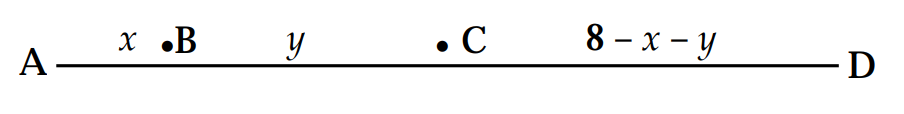
\includegraphics[width=0.5\linewidth]{figs/line1.png}
%   \end{center}

% The length of $AB$ must be less than 8 cm, and the
% length of $BC$ must be less than 8 cm too. In addition, their also must be less than the total
% length of the original segment, so $AB + BC$ is less than 8 cm. Thus, $x$ and $y$ should satisfy the following inequalities:
% \[
% \begin{cases}
%     x < 8 \\
%     y < 8 \\
%     x+y < 8
% \end{cases}
% \quad\Leftrightarrow \quad\begin{cases}
%     x < 8 \\
%     y < 8 \\
%     y < 8-x
% \end{cases}
% \]

% The shaded region ($QRS$) will be our sample space:
% \begin{center}
%     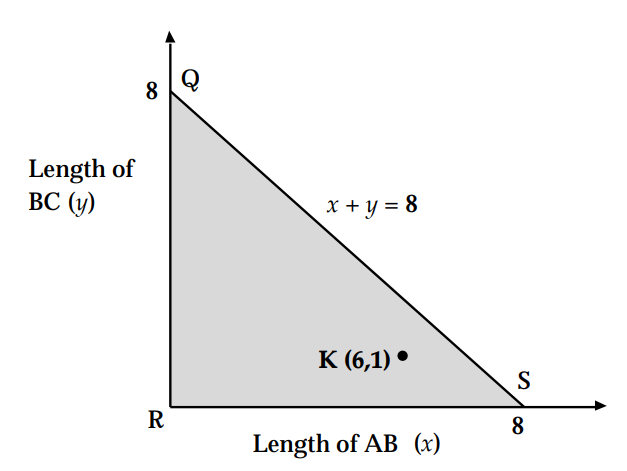
\includegraphics[width=0.4\linewidth]{figs/line2.png}
% \end{center}
% with the area $\dfrac{8\cdot 8 }{2}=32$. 

% Now, for a triangle with sides $x$, $y$, $8-x-y$ to exist, the following inequalities must hold:
% \[
% \begin{cases}
%     AB+BC>CD\\
%     AB+CD>BC\\
%     BC+CD>AB
% \end{cases}\quad\Leftrightarrow\quad
% \begin{cases}
%     x + y > 8 - x - y \\
%     x + (8 -x -y) > y\\
%     y + (8 - x - y) > x 
% \end{cases}
% \]
% which simplify to:
% \[
% \begin{cases}
%     y>4-x\\
%     y<4\\
%     x<4
% \end{cases}
% \]

% Drawing the region determined by these inequalities (i.e. the set of all $(x,y)$ points satisfying them), we get the following triangle $EFG$:
% \begin{center}
%     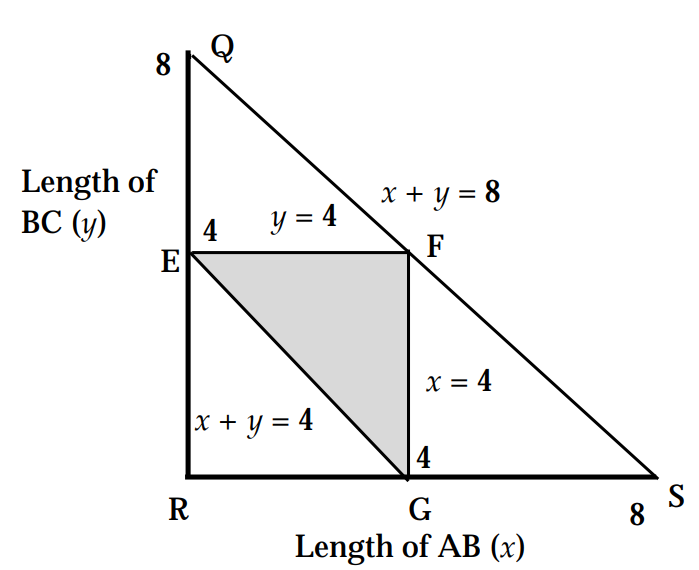
\includegraphics[width=0.36\linewidth]{figs/line3.png}
% \end{center}

% Therefore, the probability that 3 randomly selected segments will form a triangle is $\dfrac{8}{32}=0.25$.


% \end{solution}


% \smallskip

% \begin{solution}
% Let $X$ denote the number on the die. After Vahe doing the magic, the possible values $X$ can take are $2$ and $6$ each with probability $\dfrac{1}{6}$, and $3$ and $5$ each with probability $\dfrac{2}{6}$. In other words, the PMF of $X$ is:
% \[
% \PP(X=k) = \begin{cases}
%     1/6, & k\in\{2,6\} \\
%     2/6, & k\in\{3,5\} \\
%     0, & \text{otherwise}
% \end{cases}
% \]

% Therefore,
% \[
% \mathbb{E}(X) = 2 \cdot \dfrac{1}{6}  + 3 \cdot \dfrac{2}{6} + 5 \cdot \dfrac{2}{6} + 6 \cdot \dfrac{1}{6}   = 4.
% \]

% To calculate $\operatorname{Var}(X)=\mathbb{E}(X^2) - (\mathbb{E}(X))^2$, we should also calculate $\mathbb{E}(X^2)$:
% \begin{align*}
%     & \mathbb{E}(X^2) = 2^2 \cdot \dfrac{1}{6}  + 3^2 \cdot \dfrac{2}{6} + 5^2 \cdot \dfrac{2}{6} + 6^2 \cdot \dfrac{1}{6}   = 18, \\
%     & \operatorname{Var}(X) =\mathbb{E}(X^2) - (\mathbb{E}(X))^2= 18 - 4^2 = 2.
% \end{align*}

% \end{solution}

% \smallskip

% \begin{solution}
% \begin{enumerate}
%     \item[a) ] With the same steps as in the previous problem,
%     \begin{align*}
%     & \mathbb{E}(X) = \int_{-\infty}^\infty xf(x)\,dx
%                      = \int_{0}^1 x\cdot 2x \, dx
%                      = \dfrac{2}{3} x^3\bigg\vert_{0}^{1} = \dfrac{2}{3},
%     \\
%     & \mathbb{E}(X^2) = \int_{-\infty}^\infty x^2f(x)\,dx
%                      = \int_{0}^1 x^2\cdot 2x \, dx
%                      = \dfrac{2}{4} x^4\bigg\vert_{0}^{1} = \dfrac{1}{2},
%     \\
%     & \operatorname{Var}(X) =\mathbb{E}(X^2) - (\mathbb{E}(X))^2= \dfrac{1}{2}-\left(\dfrac{2}{3}\right)^2 = \dfrac{1}{18}.
%     \end{align*}
    
%     \item[b) ] Since we already have $\mathbb{E}(X)$ and since expectation is a linear function:
%     \[
%     \mathbb{E}(2X) = 2 \cdot \mathbb{E}(X) = \dfrac{4}{3},
%     \]
%     and since $\operatorname{Var}(aX)=a^2\cdot \operatorname{Var}(X)$ for all $a\in\R$,
%     \[
%     \operatorname{Var}(2X) = 4\cdot\operatorname{Var}(X) = \dfrac{2}{9}.
%     \]
        
%     \item[c) ] By the same logic, due to the linearity of expectation,
%     \[
%     \mathbb{E}(2X+7)=\mathbb{E}(2X)+7= 7\dfrac{4}{3}.
%     \]

%     As for $\operatorname{Var}(2X+7)$, after adding $7$ to $2X$, all of its values, as well as its expectation, increase by the same amount; therefore, its variance (the average squared distance between its values and their mean) should not change after adding $7$. Indeed,
%     \[
%     \operatorname{Var}(2X+7) = \mathbb{E}\big((2X+7 - \mathbb{E}(2X+7))^2\big) 
%      = \mathbb{E}\big((2X+7 - \mathbb{E}(2X) - 7)^2\big) 
%      = \mathbb{E}\big((2X- \mathbb{E}(2X) )^2\big),
%     \]
%     which equals $\operatorname{Var}(2X) = \dfrac{2}{9}$ by its definition.
    
% \end{enumerate}

% \end{solution}
